\section{Introduction}

% notion of realism, the things that we want to show. Say that there is no
% single way on how to describe water and that it is all approximations. Talk
% about the PhD thesis on the water rendering

Although water covers most of the earth's surface\footnote{Approximately 71\%
\autocite{howard2016how}} it still remains an open problem in both mathematics
and physics. There is no single solution available and approximations have to be
made. The topic is broad and complex involving subjects ranging form fast
Fourier transforms to Lagrangian and Eulerian simulations. The purpose of this
report is to present interesting water models we found in the literature and
explain how we implemented one. This document also gives our vision for further
work, namely which model should be used or avoided. In order to read this
document the reader should be familiar with the rendering pipeline and its
programmable parts. More than enough background information can be found in
\autocite{RTR3}.

We begin this report by presenting the different water models and candidate
applications in \autoref{sec:water_models}. Then we explain how we implemented
the \textit{Gerstner Wave} model in \autoref{sec:simple_gerstner_waves} and
provide performance and visual results in
\autoref{sec:performance_visual_results}. These are analyzed and discussed in
\autoref{sec:discussion}. Finally we conclude this report and give our vision
for further work in \autoref{sec:conclusion}.

\autoref{fig:anno} shows an example of an unknown real-time water model
implemented in the upcoming game \textit{Anno 1800}, developed by Blue Byte.

\begin{figure}[ht]
    \centering
    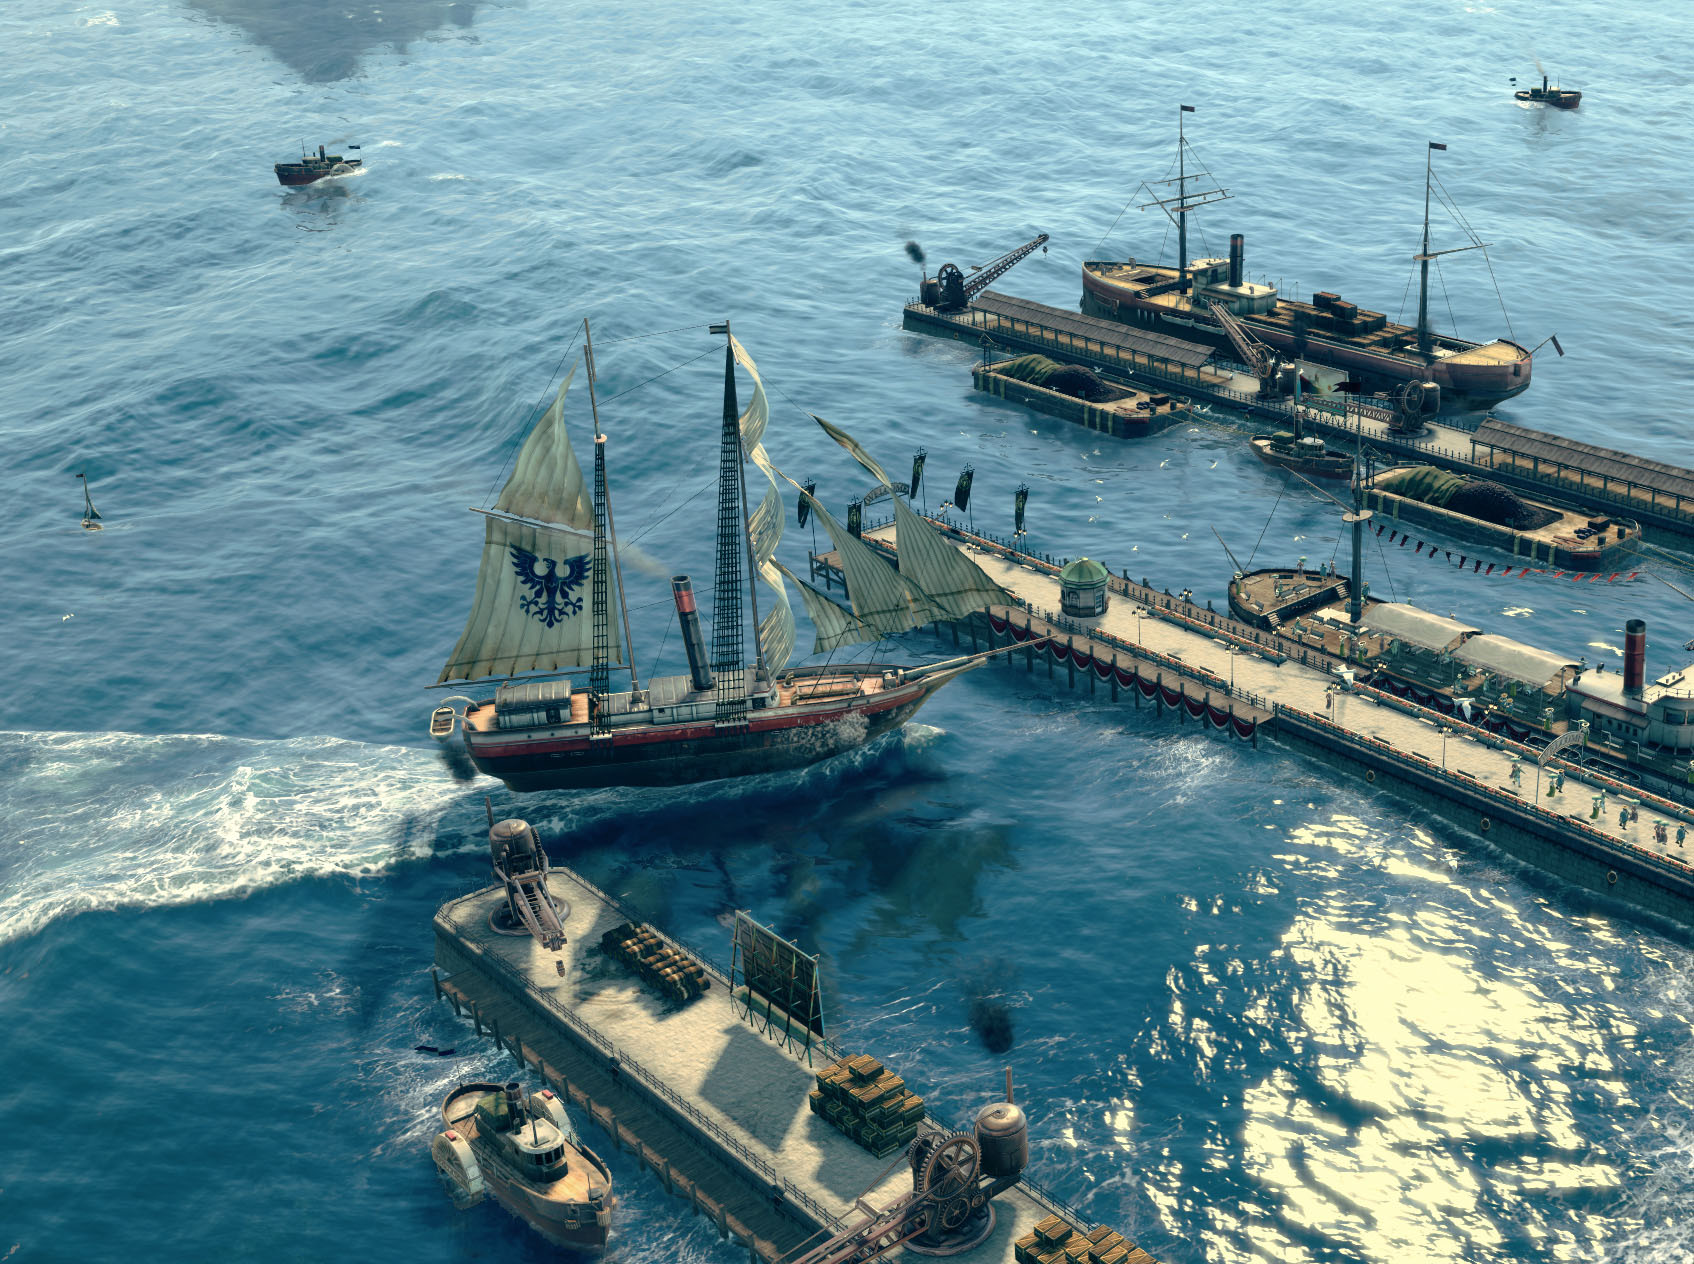
\includegraphics[height=5cm]{anno_1800.jpg}
    \caption{Harbour view from \textit{Anno 1800}. Source:
    \href{https://forum.quartertothree.com/t/anno-1800-city-building-in-the-industrial-revolution/131265/12}{\url{forum.quartertothree.com}}}\label{fig:anno}
\end{figure}
